\section{Casi d'uso}
I casi d'uso seguenti emergono da un'attenta analisi degli \textit{Analisti} del gruppo \GroupName{} rivolta al capitolato e da un'approfondita discussione con il proponente \Proponente{}. Gran parte dei casi d'uso sono stati dedotti grazie all'esperienza derivata dall'utilizzo di \glossario{ActiveAdmin}, un progetto analogo a \ProjectName{} basato su \glossario{Ruby on Rails}.\\
Ogni caso d'uso è identificato univocamente e in modo gerarchico tramite una codifica nella forma:

\begin{center}

\textit{UC[codice dell'ambito][codice univoco del padre],[codice progressivo del figlio]}

\end{center} 

dove il \textbf{codice dell'ambito} può assumere i seguenti valori:

\begin{itemize}

	\item \textbf{U} - ambito utente, che comprende sia l'utente normale che l'\textit{admin} di una applicazione generata da \ProjectName{};
	\item \textbf{S} - ambito sviluppatore.

\end{itemize}

\subsection{Ambito Utente}

\subsubsection{UC1: MaaP's Application}
		
Inserimento Immagine Base
		%\begin{figure}
%			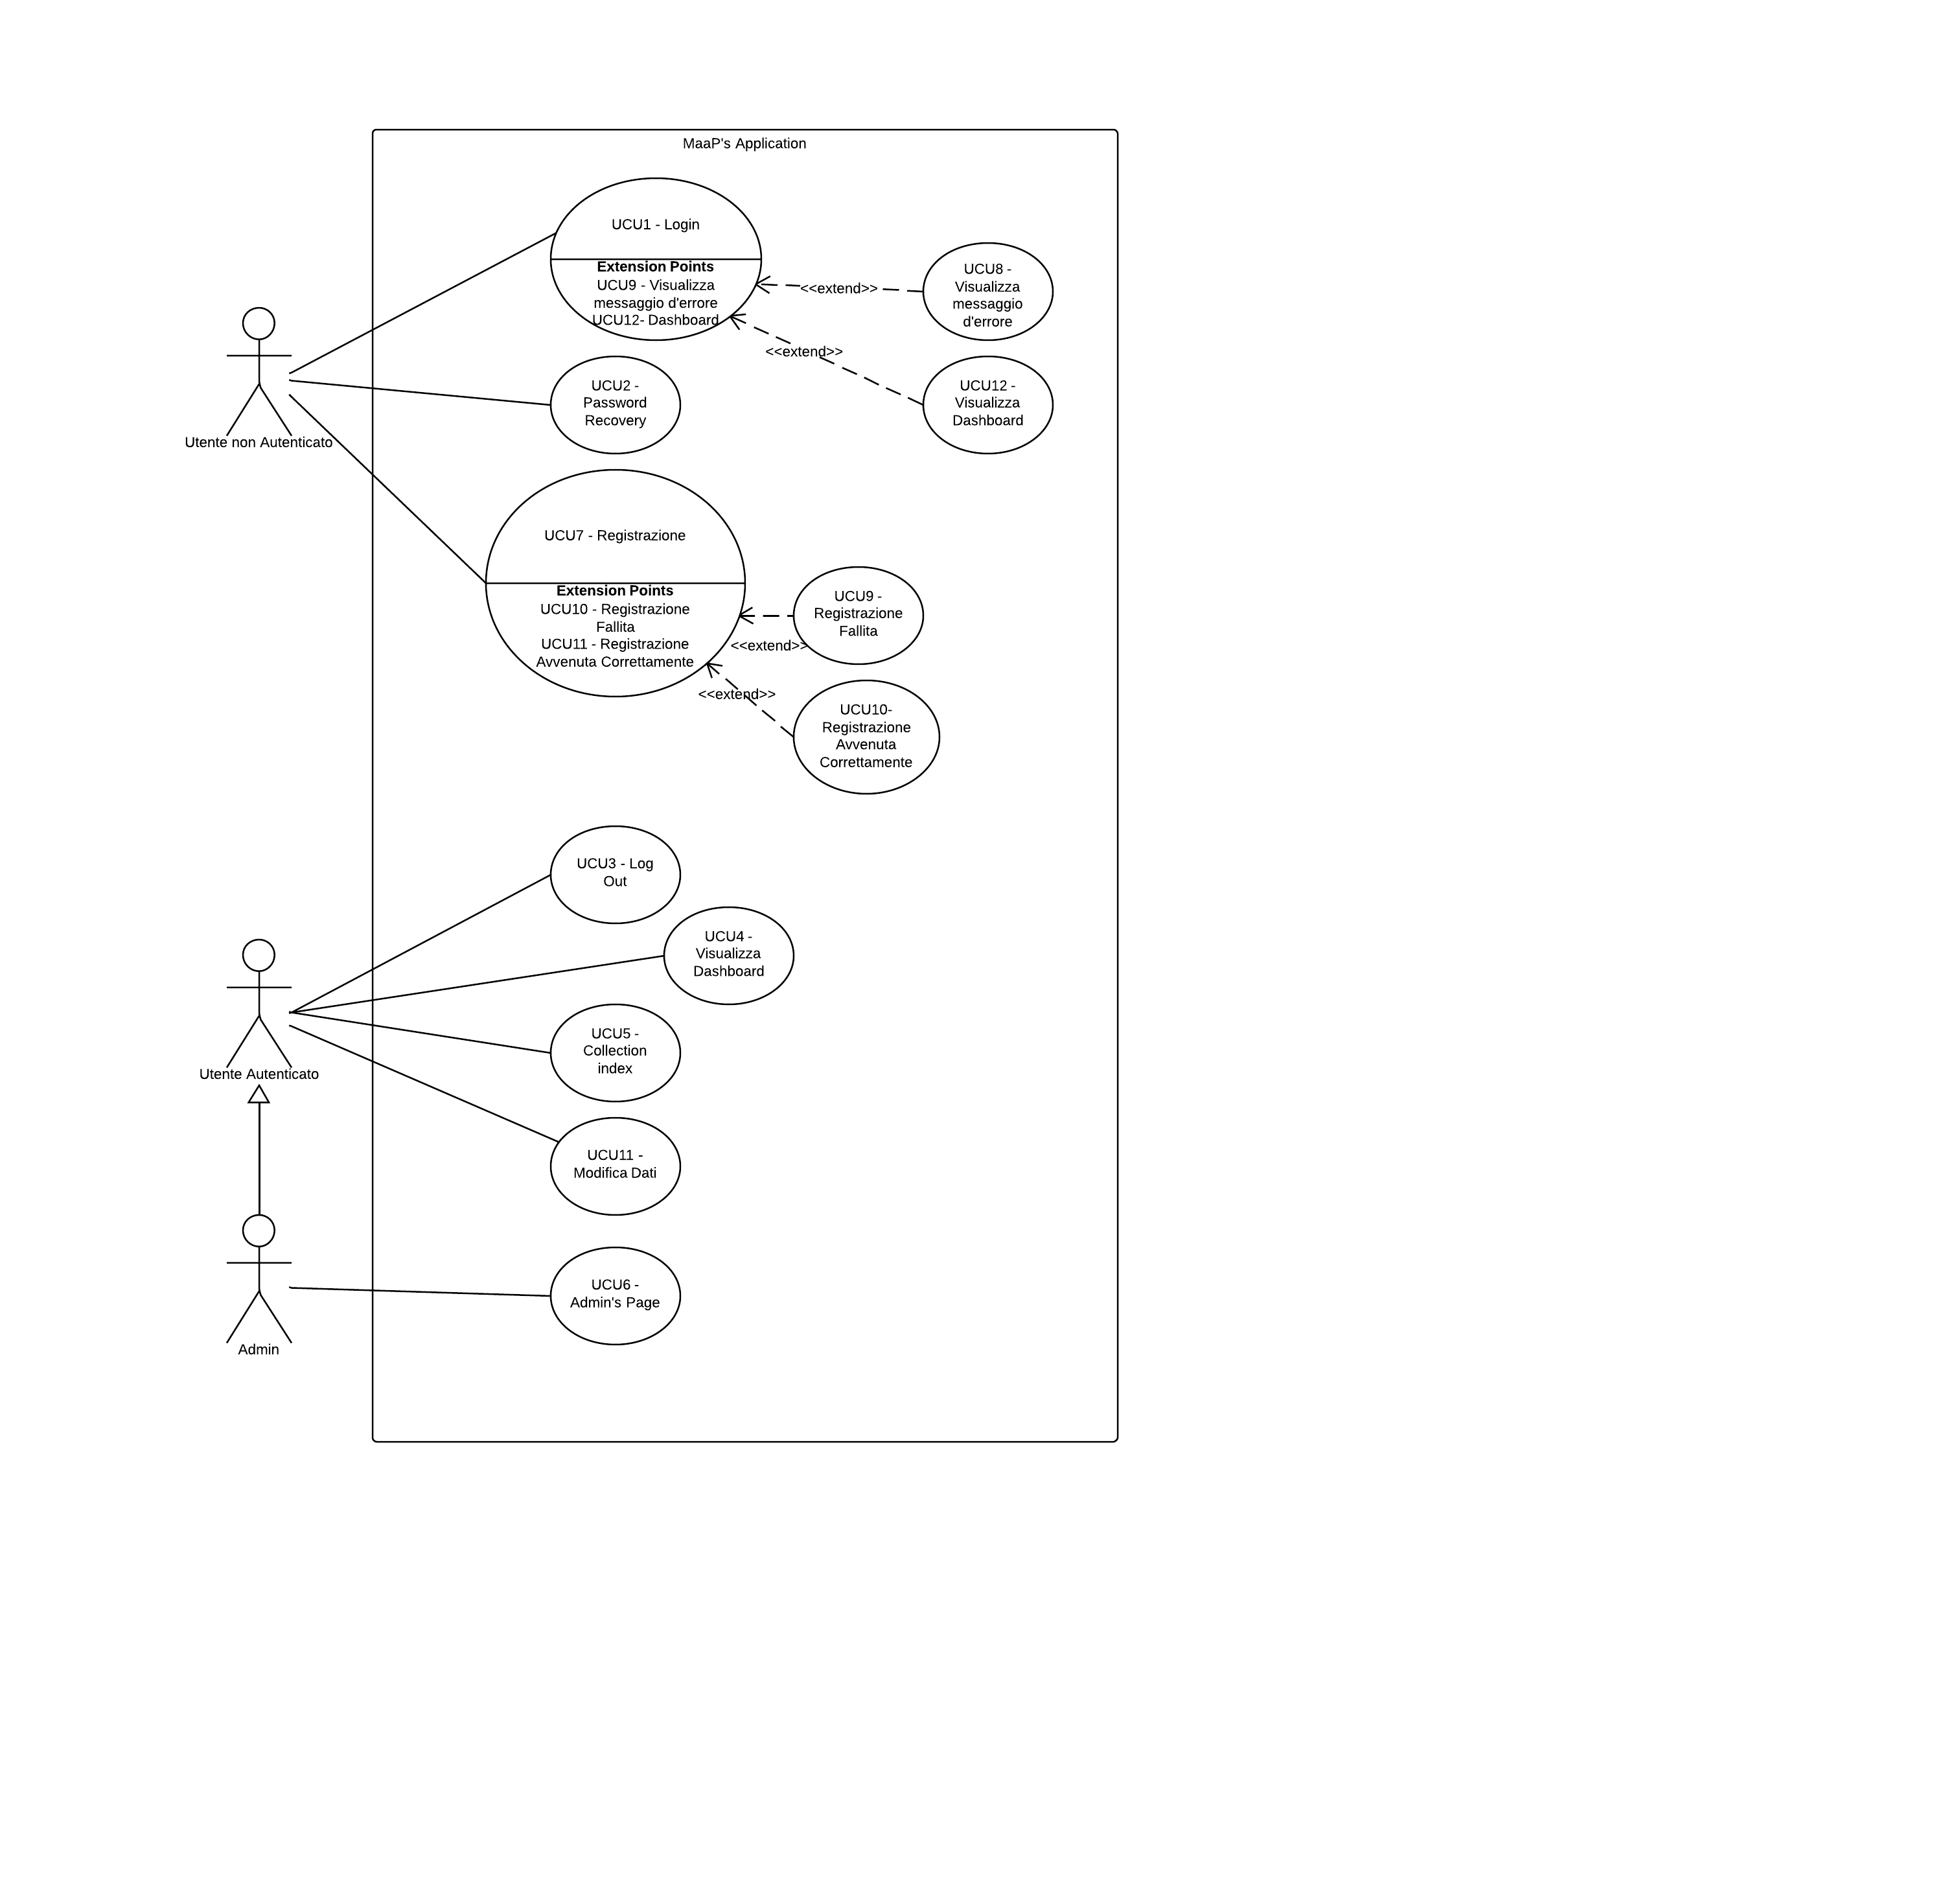
\includegraphics[scale=0.3]{UML/UCU - Maap's Application.png} % Immagine salvata in cartella da definire in norme.
%													% L'mmagine ha lo Stesso nome UCx.x corrispondente
%			\caption{UCU - MaaP's Application} % Didascalia figura, deve avere lo stesso nome dell'UCx.x
%		\end{figure}
			
		%Tabella 
			\begin{table}[h]
			\begin{longtabu}{  c | X  }
						
			\hline
			\multicolumn{2}{ | c | }{ \cellcolor[gray]{0.9} \textbf{UCU - MaaP's Application}} \\ 
			\hline
			
			 & \\
			
			\textbf{Attori Primari} & Utente non autenticato, Utente autenticato, admin \\
    			
    			\textbf{Attori Secondari} &  \\
    			
    			\textbf{Scopo e Descrizione} & L'Utente non autenticato può autenticarsi inserendo le credenziali nell'apposito form e
    			recuperare le stesse qualora le abbia perse. L'Utente autenticato in qualsiasi punto dell'applicazione può accedere alle
    			seguenti funzionalità: - può accedere alla Dashboard -può effettuare il Log Out - può scegliere una qualsiasi collection
    			presente L'Utente Admin eredita le funzionalità dell'Utente Autenticato ed in più accedere alla sezione "Admin" nella
    			quale può creare o modificare un nuovo utente. \\ 
    			
    			\textbf{Precondizioni}  & 
    			L'Applicazione generata dal framework Maap, è disponibile all'Utente e pronta all'uso ed è stato creato un account
    			dell'utente sul database. \\ 
    			
    			\textbf{Postcondizioni} &
    			Il Sistema risponde alle richieste dell'utente in maniera corretta. \\
    			
    			\textbf{Flusso Principale} & 
    	
    				1. L’Utente non autenticato può effettuare il login (UCU1); \newline
    				2. L’Utente non autenticato può recuperare la password dimenticata (UCU2); \newline
    				3. L’Utente Autenticato può effettuare il logout (UCU3); \newline
    				4. L’Utente Autenticato può accedere alla Dashboard (UCU4); \newline
    				5. L’Utente Autenticato può scegliere una qualsiasi collection presente (UCU5); \newline
    				6. L'Utente Admin può accedere alla Admin Page (UCU6).
    			 \\
    				
    			\textbf{Scenari Alternativi} & . \\
    			
    				% qui non puoi fare un itemize perchè la numerazione è prefissata in requisteak.
  
  			\end{longtabu}
			\end{table}  			 			